%\documentclass{article}
%
%\usepackage{tikz}
%\usepackage{tikz-3dplot}
%\usetikzlibrary{calc}
%\usetikzlibrary{patterns}
%\usetikzlibrary{intersections}
%\usetikzlibrary{arrows}
%\tikzset{>=latex}
%
%\begin{document}
%
%\begin{figure}[!h]
%\begin{center}
\footnotesize
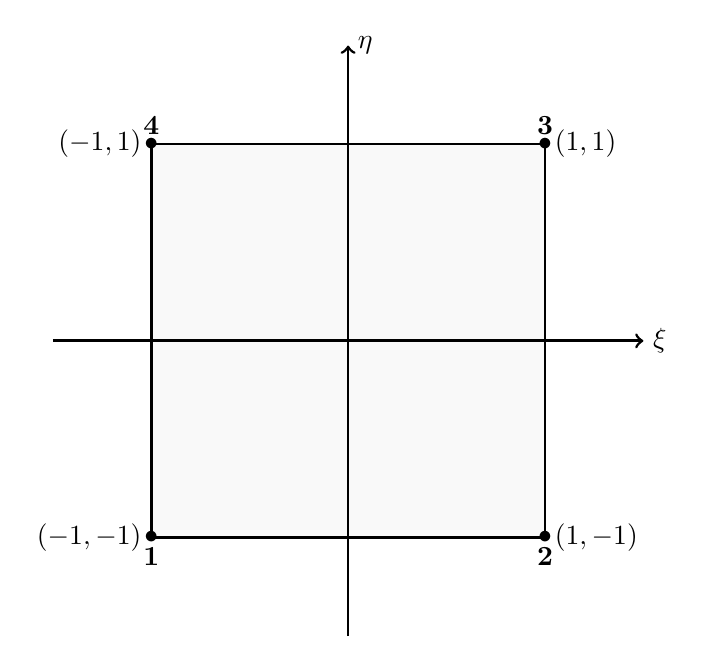
\begin{tikzpicture}[scale = 2.5]
	\coordinate[](a) at (-1,-1);
	\coordinate[](b) at (1,-1);	
	\coordinate[](c) at (1,1);
	\coordinate[](d) at (-1,1);
	
	\coordinate[](aa) at (-1.5, 0);	
	\coordinate[](bb) at (1.5, 0);
	\coordinate[](cc) at (0,-1.5);
	\coordinate[](dd) at (0,1.5);

	% Element
	\filldraw[fill=gray!5!white, line width=1pt, draw=black] 
	(a) -- (b) -- (c) -- (d) -- cycle;
	\fill[black] node at (a) {$\bullet$};
	\fill[black] node at (b) {$\bullet$};
	\fill[black] node at (c) {$\bullet$};
	\fill[black] node at (d) {$\bullet$};	

	%% Axis
	\draw [->,line width=1.0pt,black] (aa) -- (bb);
	\draw [->,line width=1.0pt,black] (cc) -- (dd);
	\node[black,right] at (bb) {$\xi$};
	\node[black,right] at (dd) {$\eta$};
	
	%% Node numeration
	\node[black, below] at (a) {$\mathbf{1}$};
	\node[black, left] at (a) {$(-1,-1)$};
	%
	\node[black, below] at (b) {$\mathbf{2}$};
	\node[black, right] at (b) {$(1,-1)$};
	%
	\node[black, above] at (c) {$\mathbf{3}$};
	\node[black, right] at (c) {$(1,1)$};
	%
	\node[black, above] at (d) {$\mathbf{4}$};
	\node[black, left] at (d) {$(-1,1)$};
	
\end{tikzpicture}
%\end{center}
%\caption{Reference Element}
%\end{figure}
%
%\end{document}